%!TEX root = ../../book_ML.tex
\chapter{Phân tích giá trị suy biến}
% \chapter{Singular value decomposition}
\label{cha:svd}
\section{Giới thiệu}
\index{phân tích giá trị suy biến -- singular value decomposition}
\index{singular value decomposition -- phân tích giá trị suy biến}
Nhắc lại bài toán chéo hoá ma trận: Một ma trận vuông $\mathbf{A} \in \mathbb{R}^{n\times n}$ gọi là {chéo hoá được} nếu tồn tại ma trận đường chéo $\mathbf{D}$ và ma trận khả nghịch $\mathbf{P}$ sao cho:
\begin{equation}
\label{eqn:26_1}
\mathbf{A} = \mathbf{P} \mathbf{D} \mathbf{P}^{-1}
\end{equation}
% Số lượng phần tử khác không của ma trận đường chéo $\mathbf{D}$ chính là hạng của ma trận $\mathbf{A}$.
Nhân cả hai vế của \eqref{eqn:26_1} với $\mathbf{P}$ ta có
\begin{equation}
\label{eqn:26_2}
\mathbf{AP} = \mathbf{PD}
\end{equation}
Gọi $\mathbf{p}_i, \mathbf{d}_i$ lần lượt là cột thứ $i$ của ma trận
$\mathbf{P}$ và $\mathbf{D}$. Vì mỗi cột của vế trái và vế phải
của~\eqref{eqn:26_2} phải bằng nhau, ta cần có
\begin{equation}
\label{eqn:26_3}
\mathbf{Ap}_i = \mathbf{Pd}_i = d_{ii}\mathbf{p}_i
\end{equation}
với $d_{ii}$ là phần tử thứ $i$ của $\mathbf{d}_i$. Dấu bằng thứ hai xảy ra vì
$\mathbf{D}$ là ma trận đường chéo, tức $\mathbf{d}_i$ chỉ có thành phần
$d_{ii}$ khác không. Biểu thức \eqref{eqn:26_3} chỉ ra rằng mỗi phần tử $d_{ii}$
phải là một {trị riêng} của $\mathbf{A}$ và mỗi vector cột $\mathbf{p}_i$ phải
là một {vector riêng} của $\mathbf{A}$ ứng với trị riêng $d_{ii}$.

\index{phân tích riêng -- eigen decomposition}
\index{eigen decomposition -- phân tích riêng}

Cách phân tích một ma trận vuông thành nhân tử như \eqref{eqn:26_1} còn được gọi
là \textit{phân tích riêng} (eigen decomposition). Đáng chú ý, không phải lúc nào cũng tồn tại cách phân tích này cho một ma trận bất kỳ. Nó chỉ tồn
tại nếu ma trận $\mathbf{A}$ có $n$ vector riêng độc lập tuyến tính, tức ma trận $\mathbf{P}$ khả nghịch. Thêm nữa, cách phân
tích này không phải là duy nhất vì nếu $\mathbf{P}, \mathbf{D}$ thoả mãn
\eqref{eqn:26_1} thì $k\mathbf{P}, \mathbf{D}$ cũng thoả mãn với $k$ là một số
thực khác không bất kỳ.

Việc phân tích một ma trận thành tích của nhiều ma trận đặc biệt khác mang lại
những ích lợi quan trọng trong bài toán gợi ý sản phẩm, giảm chiều dữ liệu, nén dữ liệu,
tìm hiểu các đặc tính của dữ liệu, giải các hệ phương trình tuyến tính,
phân cụm và nhiều ứng dụng khác.

Trong chương này, chúng ta sẽ làm quen với một trong những phương pháp phân tích
ma trận rất đẹp của đại số tuyến tính có tên là \textit{phân tích giá trị suy
biên} (singular value decomposition -- SVD)~\cite{golub1970singular}. Mọi ma
trận, không nhất thiết vuông, đều có thể được phân tích thành tích của ba ma
trận đặc biệt.

% Dưới đây, tôi sẽ phát biểu SVD cũng như các tính chất và ứng dụng điển hình của nó.

% Trước hết, chúng ta cần ôn tập lại một chút về Đại số tuyến tính. \textbf{Chú ý rằng các ma trận trong bài viết này đều được ngầm giả sử là ma trận thực}.


% \section{Một chút về Đại số tuyến tính}


% \subsection{Trị riêng và vector riêng}
% Cho một ma trận vuông $\mathbf{A} \in \mathbb{R}^{n\times n}$, nếu số vô hướng $\lambda$ và vector $\mathbf{x} \neq \mathbf{0} \in \mathbb{R}^n$ thoả mãn:

% \begin{equation}
% \mathbf{Ax} = \lambda \mathbf{x}
% \end{equation}
% thì $\lambda$ được gọi là một trị riêng của $\mathbf{A}$ và $\mathbf{x}$ được gọi là vector riêng tương ứng với trị riêng đó.

% Một vài tính chất:

% \begin{enumerate}
%     \item Nếu $\mathbf{x}$ là một vector riêng của $\mathbf{A}$ ứng với $\lambda$ thì $k\mathbf{x}, k \neq 0$ cũng là vector riêng ứng với trị riêng đó.

%     \item Mọi ma trận vuông bậc $n$ đều có $n$ trị riêng (kể cả lặp) và có thể là các số phức.

%     \item Với ma trận đối xứng, tất cả các trị riêng đều là các số thực.

%     \item Với \href{http://machinelearningcoban.com/2017/03/12/convexity/#positive-semidefinite}{\textit{ma trận xác định dương}}, tất cả các trị riêng của nó đều là các số thực dương. Với \textit{ma trận nửa xác định dương}, tất cả các trị riêng của nó đều là các số thực không âm.
% \end{enumerate}

% Tính chất cuối cùng có thể được suy ra từ định nghĩa của ma trận (nửa) xác định dương. Thật vậy, gọi $\mathbf{u} \neq \mathbf{0}$ là vector riêng ứng với một trị riêng $\lambda$ của ma trận $\mathbf{A}$ xác định dương, ta có:
% \begin{equation}
% \mathbf{Au} = \lambda \mathbf{u} \Rightarrow \mathbf{u}^T\mathbf{Au} = \lambda \mathbf{u}^T\mathbf{u} = \lambda \|\mathbf{u}\|_2^2
% \end{equation}

% Vì $\mathbf{A}$ là nửa xác định dương nên với mọi $\mathbf{u} \neq \mathbf{0}$: $\mathbf{u}^T\mathbf{Au} \geq 0$; $\mathbf{u} \neq 0$ nên $\|\mathbf{u}\|_2^2 > 0$. Từ đó suy ra $\lambda$ là một số không âm.


% \subsection{Hệ trực giao và trực chuẩn}

% Một hệ cơ sở $\{\mathbf{u}_1, \mathbf{u}_2,\dots, \mathbf{u}_m \in \mathbb{R}^m\}$ được gọi là \textit{trực giao} (orthogonal) nếu mỗi vector là khác 0 và tích của hai vector khác nhau bất kỳ bằng 0:

% \begin{equation}
% \mathbf{u}_i \neq \mathbf{0}; ~~ \mathbf{u}_i^T \mathbf{u}_j = 0 ~ \forall ~1 \leq i \neq j \leq m
% \end{equation}

% Một hệ cơ sở $\{\mathbf{u}_1, \mathbf{u}_2,\dots, \mathbf{u}_m \in \mathbb{R}^m\}$ được gọi là \textit{trực chuẩn} (orthonormal) nếu nó là một hệ \textit{trực giao} và độ dài Euclidean (norm 2) của mỗi vector bằng 1:

% \begin{eqnarray}
% \label{eqn:26_4}
% \mathbf{u}_i^T \mathbf{u}_j = \left\{
% \begin{matrix}
%     1 & \text{if} &i = j \\\
%     0 & \text{otherwise}
% \end{matrix}
% \right.
% \end{eqnarray}

% Gọi $\mathbf{U} = [\mathbf{u}_1, \mathbf{u}_2,\dots, \mathbf{u}_m]$ với $\{\mathbf{u}_1, \mathbf{u}_2,\dots, \mathbf{u}_m \in \mathbb{R}^m\}$ là \textit{trực chuẩn}, thế thì từ \eqref{eqn:26_4} có thể suy ra ngay:

% \begin{equation}
% \mathbf{UU}^T = \mathbf{U}^T\mathbf{U} = \mathbf{I}
% \end{equation}

% trong đó $\mathbf{I}$ là ma trận đơn vị bậc $m$. Ta gọi $\mathbf{U}$ là \textit{ma trận trực giao} (orthogonal matrix). \textit{Ma trận loại này không không được gọi là ma trận trực chuẩn, không có định nghĩa cho ma trận trực chuẩn.}

% Một vài tính chất:

% \begin{enumerate}

%     \item $\mathbf{U}^{-1} = \mathbf{U}^T$: nghịch đảo của một ma trận trực giao chính là chuyển vị của nó.

%     \item Nếu $\mathbf{U}$ là ma trận trực giao thì chuyển vị của nó $\mathbf{U}^T$ cũng là một ma trận trực giao.

%     \item Định thức (determinant) của ma trận trực giao bằng $1$ hoặc $-1$. Điều này có thể suy ra từ việc $\det(\mathbf{U}) = \det(\mathbf{U}^T)$ và $\det(\mathbf{U}) \det(\mathbf{U}^T) = \det(\mathbf{I}) = 1$.

%     \item Ma trận trực giao thể hiện cho phép xoay (rotate) một vector. Giả sử có hai vector $\mathbf{x,y} \in \mathbb{R}^m$ và ma trận trực giao $\mathbf{U} \in \mathbb{R}^{m \times m}$. Dùng ma trận này để xoay hai vector trên ta được $\mathbf{Ux}, \mathbf{Uy}$. Tích vô hướng của hai vector mới là:
%     \begin{equation}
%     (\mathbf{Ux})^T (\mathbf{Uy}) = \mathbf{x}^T \mathbf{U}^T \mathbf{Uy} = \mathbf{x}^T\mathbf{y}
%     \end{equation}
%     như vậy \textit{phép xoay không làm thay đổi tích vô hướng giữa hai vector}.

%     \item Giả sử $\hat{\mathbf{U}} \in \mathbb{R}^{m \times r}, r < m$ là môt ma trận con của ma trận trực giao $\mathbf{U}$ được tạo bởi $r$ cột của $\mathbf{U}$, ta sẽ có $\hat{\mathbf{U}}^T\hat{\mathbf{U}} = \mathbf{I}_{r}$. Việc này có thể được suy ra từ \eqref{eqn:26_4}.

% \end{enumerate}


\section{Phân tích giá trị suy biến}
Để hạn chế nhầm lẫn trong các phép toán, ta sẽ ký hiệu một ma trận cùng với kích thước của nó, ví dụ $\mathbf{A}_{m \times n}$ ký hiệu một ma trận
$\mathbf{A} \in \mathbb{R}^{m \times n}$.

\subsection{Phát biểu phân tích giá trị suy biến}
\index{SVD}
% \hrule
\newnote{Phân tích giá trị suy biến (SVD)}{
Một ma trận $\mathbf{A}_{m \times n}$ bất kỳ đều có thể phân tích thành dạng:
\begin{equation}
\label{eqn:26_5}
\mathbf{A}_{m \times n} = \mathbf{U}_{m \times m}\mathbf{\bSigma}_{m \times n} (\mathbf{V}_{n \times n})^T
\end{equation}
với $\mathbf{U}, \mathbf{V}$ là các \textit{ma trận trực giao},
$\mathbf{\bSigma}$ là một ma trận đường chéo cùng kích thước với $\bA$. Các
phần tử trên đường chéo chính của $\bSigma$ là không âm và được sắp xếp theo thứ tự
giảm dần $\sigma_1 \geq \sigma_2 \geq \dots \geq\sigma_r \geq 0 = 0
= \dots = 0$. Số lượng các phần tử khác
không trong $\bSigma$ chính là hạng của ma trận $\mathbf{A}$: $r = \rank(\bA)$.
}

% \hrule

SVD của một ma trận bất kỳ luôn tồn tại\footnote{Bạn đọc có thể tìm thấy chứng
minh cho việc này tại \url{https://goo.gl/TdtWDQ}.}. Cách biểu diễn
\eqref{eqn:26_5} không là duy nhất vì ta chỉ cần đổi dấu của cả $\mathbf{U}$ và
$\mathbf{V}$ thì \eqref{eqn:26_5} vẫn thoả mãn.

Hình~\ref{fig:26_1} mô tả SVD của ma trận $\mathbf{A}_{m \times n}$ trong hai
trường hợp: $m < n$ và $m > n$. Trường hợp $m =n$ có thể xếp vào một trong hai
trường hợp trên.

% ******************************************************************************
\begin{figure}[t]
\centering
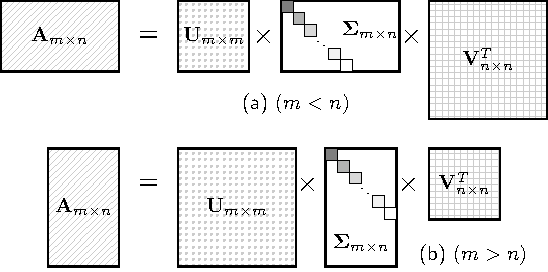
\includegraphics[width = .85\textwidth]{Chapters/07_DimemsionalityReduction/26_svd/latex/svd.pdf}
\caption[]{SVD cho ma trận $\mathbf{A}$ khi: (a) $m < n$, và (b) $m > n$. $\bSigma$ là một ma trận đường chéo với các phần tử trên đó
giảm dần và không âm. Màu xám càng đậm thể hiện giá trị càng cao. Các ô màu
trắng trên ma trận $\bSigma$ thể hiện giá trị bằng không.}
\label{fig:26_1}
\end{figure}
% ******************************************************************************
\subsection{Nguồn gốc tên gọi}
Tạm bỏ qua chiều của mỗi ma trận, từ \eqref{eqn:26_5} ta có:
\begin{eqnarray}
\mathbf{AA}^T &=& \mathbf{U}\mathbf{\bSigma} \mathbf{V}^T (\mathbf{U}\mathbf{\bSigma} \mathbf{V}^T)^T \\\
\label{eqn:26_6a}
&=& \mathbf{U}\mathbf{\bSigma} \mathbf{V}^T \mathbf{V}\mathbf{\bSigma}^T\mathbf{U}^T \\\
\label{eqn:26_6}
&=& \mathbf{U}\mathbf{\bSigma}\mathbf{\bSigma}^T\mathbf{U}^T =  \mathbf{U}\mathbf{\bSigma}\mathbf{\bSigma}^T\mathbf{U}^{-1}
\end{eqnarray}
Dấu bằng ở~\eqref{eqn:26_6a} xảy ra vì $\mathbf{V}^T\mathbf{V} = \mathbf{I}$ do
$\mathbf{V}$ là một ma trận trực giao. Dấu bằng ở~\eqref{eqn:26_6} xảy ra vì
$\bU$ là một ma trận trực giao.

\index{giá trị suy biến -- singular value}
\index{singular value -- giá trị suy biến}
\index{vector suy biến trái -- left-singular value}
\index{left-singular value -- vector suy biến trái}
\index{vector suy biến phải -- right-singular value}
\index{right-singular value -- vector suy biến phải}

Quan sát thấy rằng $\bSigma\bSigma^T$ là một ma trận đường chéo với các phần tử
trên đường chéo là $\sigma_1^2, \sigma_2^2, \dots$ Vậy~\eqref{eqn:26_6} chính
là một phân tích riêng của $\mathbf{A}\mathbf{A}^T$và $\sigma_1^2,
\sigma_2^2, \dots$ là các trị riêng của ma trận này.
Ma trận $\mathbf{A}\mathbf{A}^T$ luôn là nửa xác định dương nên các trị
riêng của nó là không âm. Căn bậc hai các trị riêng của
$\mathbf{A}\mathbf{A}^T$, $\sigma_i$, còn được gọi là \textit{giá trị suy biến} (singular value) của
$\mathbf{A}$. Tên gọi \textit{phân tích giá trị suy biến} xuất phát từ đây.

Cũng theo đó, mỗi cột của $\mathbf{U}$ là một vector riêng của
$\mathbf{A}\mathbf{A}^T$. Ta gọi mỗi cột này là một \textit{vector suy biến trái} (left-singular
vector) của $\mathbf{A}$. Tương tự, $\mathbf{A}^T\mathbf{A} =
\mathbf{V}\bSigma^T\bSigma \mathbf{V}^T$ và các cột của $\mathbf{V}$ được
gọi là các \textit{vector suy biến phải} ({right-singular vectors}) của $\mathbf{A}$.

Trong Python, để tính SVD của một ma trận, chúng ta sử dụng module
\pythoninline{linalg} của \pythoninline{numpy}:

\begin{lstlisting}[language=Python]
from __future__ import print_function
import numpy as np
from numpy import linalg as LA

m, n = 3, 4
A = np.random.rand(m, n)
U, S, V = LA.svd(A) # A = U*S*V (no V transpose here)

# checking if U, V are orthogonal and S is a diagonal matrix with
# nonnegative decreasing elements
print('Frobenius norm of (UU^T - I) =', LA.norm(U.dot(U.T) - np.eye(m)))
print('S = ', S)
print('Frobenius norm of (VV^T - I) =', LA.norm(V.dot(V.T) - np.eye(n)))
\end{lstlisting}
\newpage
Kết quả:
\begin{lstlisting}
Frobenius norm of (UU^T - I) = 4.09460889695e-16
S =  [ 1.76321041  0.59018069  0.3878011 ]
Frobenius norm of (VV^T - I) = 5.00370755311e-16
\end{lstlisting}

Lưu ý rằng biến \pythoninline{S} được trả về chỉ bao gồm các phần tử trên đường
chéo của $\bSigma$. Biến \pythoninline{V} trả về là $\mathbf{V}^T$ trong
\eqref{eqn:26_5}.

\subsection{Giá trị suy biến của ma trận nửa xác định dương}
Giả sử $\bA$ là một ma trận vuông đối xứng nửa xác định dương, ta sẽ chứng minh rằng giá trị suy biến  chính là trị riêng của nó. Thật vậy, gọi $\lambda$ là một trị riêng của $\bA$ và $\bx$ là một vector riêng ứng với trị riêng và $\|\bx\|_2 = 1$. Vì $\bA$ là nửa xác định dương, $\lambda \geq 0$.
Ta có
\begin{equation}
\bA\bx = \lambda\bx \imply \bA^T\bA\bx = \lambda\bA\bx = \lambda^2\bx
\end{equation}
Như vậy, $\lambda^2$ là một trị riêng của $\bA^T\bA \imply$ giá trị suy biến của $\bA$ chính là $\sqrt{\lambda^2} = \lambda$.

\begin{figure}[t]
\centering
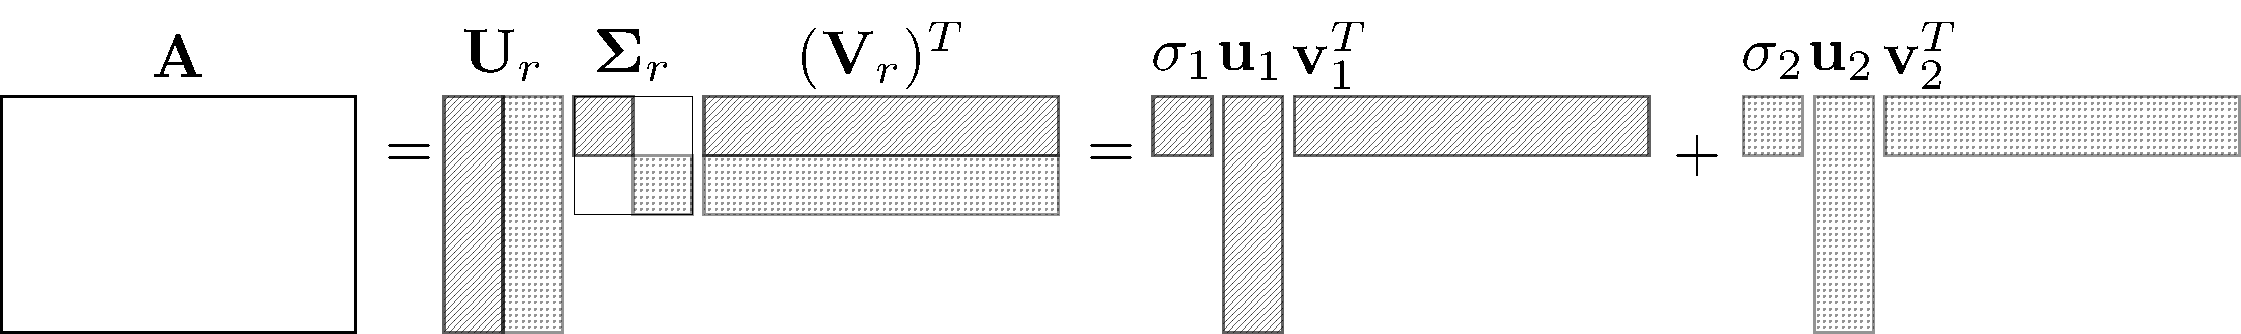
\includegraphics[width = \textwidth]{Chapters/07_DimemsionalityReduction/26_svd/latex/svd_truncated.pdf}
\caption[]{Biểu diễn \textit{compact SVD} dưới dạng tổng
các ma trận có rank bằng 1. Các khối ma trận đặt cạnh nhau thể hiện phép
nhân ma trận.}
\label{fig:26_2}
\end{figure}


\subsection{Phân tích giá trị suy biến giản lược}
Viết lại biểu thức \eqref{eqn:26_5} dưới dạng tổng của các ma trận có hạng
bằng môt:
\begin{equation}
\mathbf{A} = \sigma_1 \mathbf{u}_1 \mathbf{v}^T_1 + \sigma_2\mathbf{u}_2\mathbf{v}_2^T + \dots + \sigma_r\mathbf{u}_r\mathbf{v}_r^T
\end{equation}
với chú ý rằng mỗi $\mathbf{u}_i\mathbf{v}^T_i, 1 \leq i \leq r$, là một ma trận có hạng bằng một.

\index{SVD giản lược -- compact SVD}
\index{compact SVD -- SVD giản lược}
Trong cách biểu diễn này, ma trận $\mathbf{A}$ chỉ phụ thuộc vào $r$ cột
đầu tiên của $\mathbf{U, V}$ và $r$ giá trị khác 0 trên đường chéo của ma trận
$\bSigma$. Vì vậy ta có một cách phân tích {gọn} hơn và gọi là \textit{SVD giản lược} (compact SVD):
\begin{equation}
\mathbf{A} = {\mathbf{U}}_r{\bSigma}_r({\mathbf{V}}_r)^T
\end{equation}
với $\mathbf{U}_r, \mathbf{V}_r $ lần lượt là ma trận được tạo bởi $r$ cột đầu
tiên của $\mathbf{U}$ và $\mathbf{V}$. $\bSigma_r$ là ma trận con được tạo bởi
$r$ hàng đầu tiên và $r$ cột đầu tiên của $\bSigma$. Nếu ma trận $\mathbf{A}$ có
hạng nhỏ hơn rất nhiều so với số hàng và số cột, tức $r \ll m, n$, ta sẽ được lợi
nhiều về việc lưu trữ. Hình~\ref{fig:26_2} là một ví dụ minh hoạ với $m = 4, n = 6, r = 2$.
% <hr>
% <div class="imgcap">
% <img src ="/assets/26_svd/svd_truncated.png" align = "center" width = "800">
% </div>

% <div class = "thecap" align = "left">Hình 2: Biểu diễn SVD dạng thu gọn và biểu diễn ma trận dưới dạng tổng các ma trận có rank bằng 1.</div>
% <hr>

\index{SVD cắt ngọn -- truncated SVD}
\index{truncated SVD -- SVD cắt ngọn}
\subsection{Phân tích giá trị suy biến cắt ngọn}
Nhắc lại rằng các giá trị trên đường chéo chính của $\bSigma$ là không âm
và giảm dần $\sigma_1 \geq \sigma_2 \geq \dots, \geq \sigma_r \geq 0 = 0 = \dots
= 0$. Thông thường, chỉ một lượng nhỏ các $\sigma_i$ mang giá trị lớn, các giá
trị còn lại nhỏ và gần không. Khi đó ta có thể xấp xỉ ma trận $\mathbf{A}$
bằng tổng của $k < r$ ma trận có hạng bằng một:
\begin{equation}
\mathbf{A} \approx \mathbf{A}_k = \mathbf{U}_k \bSigma_k (\mathbf{V}_k)^T = \sigma_1 \mathbf{u}_1 \mathbf{v}^T_1 + \sigma_2\mathbf{u}_2\mathbf{v}_2^T + \dots + \sigma_k\mathbf{u}_k\mathbf{v}_k^T
\end{equation}
Việc bỏ đi $r-k$ giá trị suy biến khác không nhỏ nhất được gọi là \textit{SVD cắt ngọn} (truncated SVD). Dưới đây là một định lý thú vị. Định lý này nói rằng sai số do cách xấp xỉ SVD cắt ngọn bằng căn bậc hai tổng bình phương của các giá trị suy biến bị cắt đi. Ở đây sai số được định nghĩa là Frobineous norm của
hiệu hai ma trận.
\begin{mytheo}{Sai số do xấp xỉ bởi SVD cắt ngọn}{truncatedsvd}
Sai số do xấp xỉ một ma trận $\bA$ có hạng $r$ bởi SVD cắt ngọn với $k < r$ phần tử là
\begin{equation}
\|\mathbf{A} - \mathbf{A}_k\|_F^2 = \sum_{i = k + 1}^r \sigma_i^2
\end{equation}
\end{mytheo}

\textit{Chứng minh:} Sử dụng tính chất $\|\mathbf{X}\|_F^2 = \text{trace}(\mathbf{X}\mathbf{X}^T)$ và
$\text{trace}(\mathbf{XY}) = \text{trace}(\mathbf{YX})$ với mọi ma trận
$\mathbf{X, Y}$ ta có:
\begin{eqnarray}
% \label{eqn:26_9}
\nonumber
\|\mathbf{A} - \mathbf{A}_k\|_F^2 & = & \left\|\sum_{i = k + 1}^r \sigma_i
\mathbf{u}_i\mathbf{v}_i^T \right\|_F^2
=  \text{trace}\left\{ \left(\sum_{i = k + 1}^r \sigma_i \mathbf{u}_i\mathbf{v}_i^T\right)
\left(\sum_{j = k + 1}^r \sigma_j \mathbf{u}_j\mathbf{v}_j^T\right)^T
\right\}  \\\
\label{eqn:26_12}
&=& \text{trace}\left\{ \sum_{i = k + 1}^r \sum_{j = k + 1}^r \sigma_i\sigma_j \mathbf{u}_i\mathbf{v}_i^T \mathbf{v}_j \mathbf{u}_j^T
\right\}
= \text{trace}\left\{ \sum_{i = k + 1}^r  \sigma_i^2\mathbf{u}_i\mathbf{u}_i^T
\right\} \\\
\label{eqn:26_13}
&=& \text{trace}\left\{ \sum_{i = k + 1}^r  \sigma_i^2\mathbf{u}_i^T\mathbf{u}_i
\right\}  \\\
\label{eqn:26_15}
&=& \text{trace}\left\{ \sum_{i = k + 1}^r  \sigma_i^2
\right\}  = \sum_{i = k + 1}^r \sigma_i^2
\end{eqnarray}
Dấu bằng thứ hai ở \eqref{eqn:26_12} xảy ra vì $\mathbf{V}$ có các cột vuông góc với nhau.
Dấu bằng ở \eqref{eqn:26_13} xảy ra vì hàm $\text{trace}$ có tính chất giao hoán.
Dấu bằng ở \eqref{eqn:26_15} xảy ra vì biểu thức trong dấu ngoặc là một số vô hướng. \dpcm

Thay $k = 0$ ta sẽ có
\begin{equation}
\label{eqn:26_16}
\|\mathbf{A}\|_F^2 = \sum_{i = 1}^r \sigma_i^2
\end{equation}
\index{xấp xỉ hạng thấp -- low-rank approximation}
\index{low-rank approximation -- xấp xỉ hạng thấp}
Từ đó
\begin{equation}
\label{eqn:26_17}
\frac{\|\mathbf{A} - \mathbf{A}_k\|_F^2}{\|\mathbf{A}\|_F^2} = {\frac{\sum_{i =
k + 1}^r \sigma_i^2}{\sum_{j = 1}^r \sigma_j^2}}
\end{equation}
Như vậy, \textit{sai số do xấp xỉ càng nhỏ nếu các giá trị suy biến bị
cắt càng nhỏ so với các giá trị suy biến được giữ lại.}
Đây là một định lý quan trọng giúp xác định việc xấp xỉ ma trận dựa trên lượng
thông tin muốn giữ lại. Ở đây, {lượng thông tin} được định nghĩa
là tổng bình phương của giá trị suy biến. Ví dụ, nếu muốn giữ lại ít nhất
90\% lượng thông tin trong $\mathbf{A}$, trước hết ta tính $\sum_{j = 1}^r
\sigma_j^2$, sau đó chọn $k$ là số nhỏ nhất sao cho
\begin{equation}
\frac{\sum_{i = 1}^k \sigma_i^2}{\sum_{j = 1}^r \sigma_j^2} \geq 0.9
\end{equation}
Khi $k$ nhỏ, ma trận $\mathbf{A}_k$ có hạng nhỏ bằng $k$
Vì vậy, SVD cắt ngọn cũng được xếp vào loại \textit{xấp xỉ hạng thấp}.


\subsection{Xấp xỉ hạng $k$ tốt nhất}

Người ta chứng minh được rằng\footnote{Singular Value Decomposition  --
Princeton (\url{https://goo.gl/hU38GF}).}
$\mathbf{A}_k$ chính là nghiệm của bài toán tối ưu sau đây:
\begin{equation}
\label{eqn:26_17}
\begin{aligned}
\min_{\mathbf{B}} &\|\mathbf{A} - \mathbf{B}\|_F \\\
\text{thoả mãn:}~ & \text{rank}(\mathbf{B}) = k
\end{aligned}
\end{equation}
và $\|\mathbf{A} - \mathbf{A}_k\|_F^2 = \sum_{i = k + 1}^r \sigma_i^2$ như đã chứng minh ở trên .

Nếu sử dụng $\ell_2$ norm của ma trận (xem Phụ lục~\ref{apd:lagrange}) thay vì
Frobenius norm để đo
sai số,
$\mathbf{A}_k$ cũng là nghiệm của bài toán tối ưu
\begin{equation}
\begin{aligned}
\min_{\mathbf{B}} &\|\mathbf{A} - \mathbf{B}\|_2 \\\
\text{thoả mãn:}~ & \text{rank}(\mathbf{B}) = k
\end{aligned}
\end{equation}
và sai số $\|\mathbf{A} - \mathbf{A}_k\|_2^2 = \sigma_{k+1}^2$. Trong đó, $\ell_2$ norm
của một ma trận được định nghĩa bởi
\begin{equation}
\|\mathbf{A}\|_2 = \max_{\|\mathbf{x}\|_2 = 1} \|\mathbf{Ax}\|_2
\end{equation}
Frobenius norm và $\ell_2$ norm là hai norm được sử dụng nhiều nhất trong ma
trận. Như vậy, xét trên cả hai norm này, SVD cắt ngọn đều cho xấp xỉ tốt nhất.
Vì vậy, SVD cắt ngọn còn được coi là \textit{xấp xỉ hạng thấp tốt nhất} ({best low-rank approximation}).



\section{Phân tích giá trị suy biến cho bài toán nén ảnh}

% \subsection{Image Compression}

%% ******************************************************************************
\begin{figure}[t]
\begin{subfigure}{0.325\textwidth}
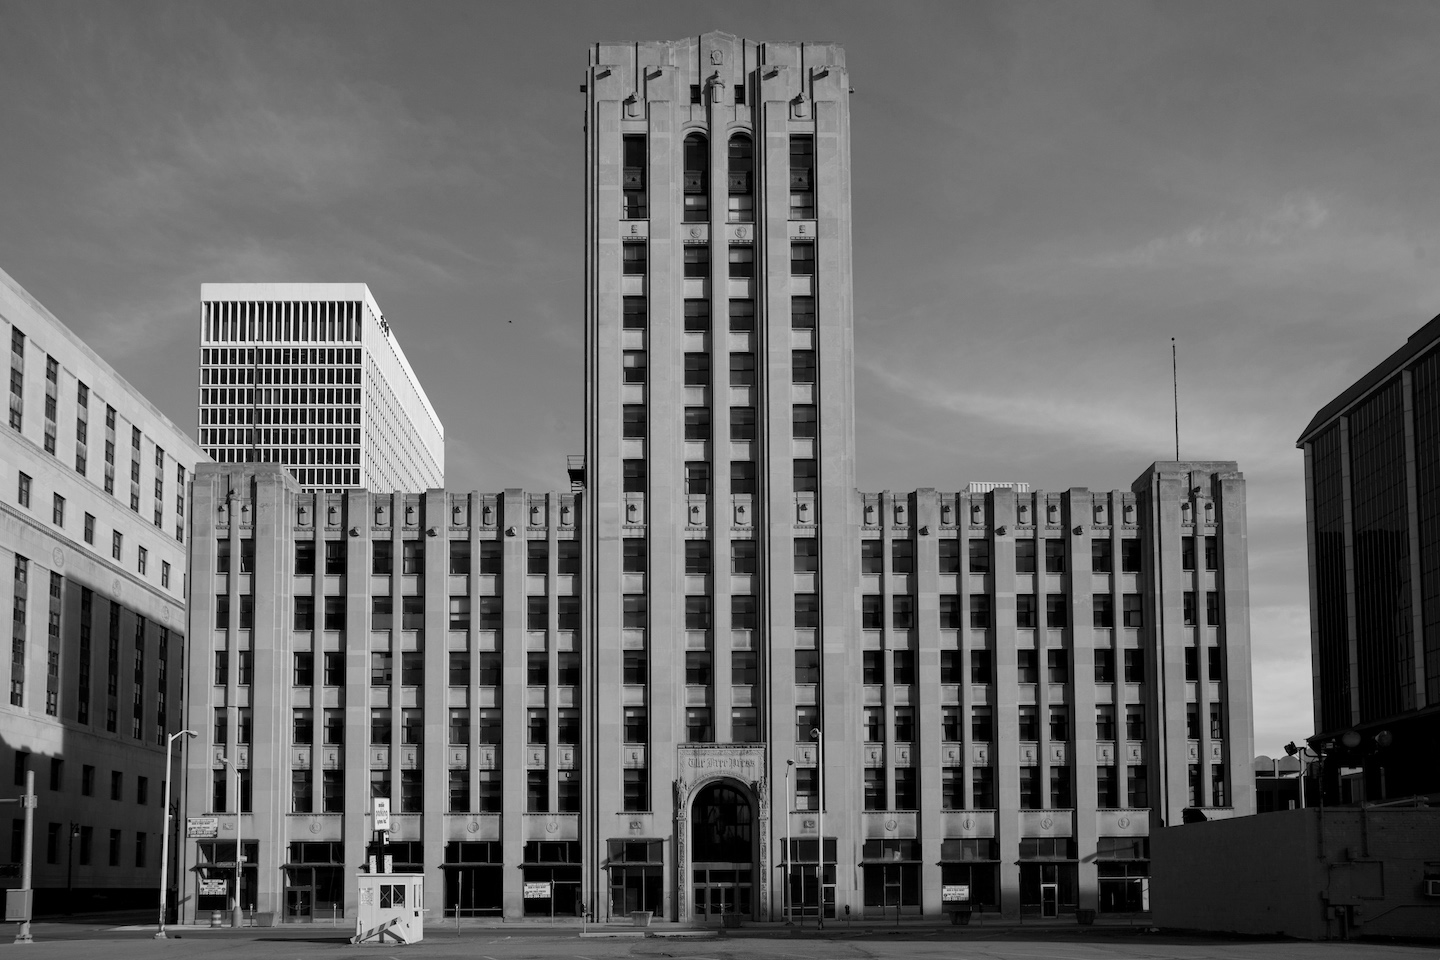
\includegraphics[width=0.95\linewidth]{Chapters/07_DimemsionalityReduction/26_svd/original.png}
\caption{}
\label{fig:26_3a}
\end{subfigure}
\begin{subfigure}{0.325\textwidth}
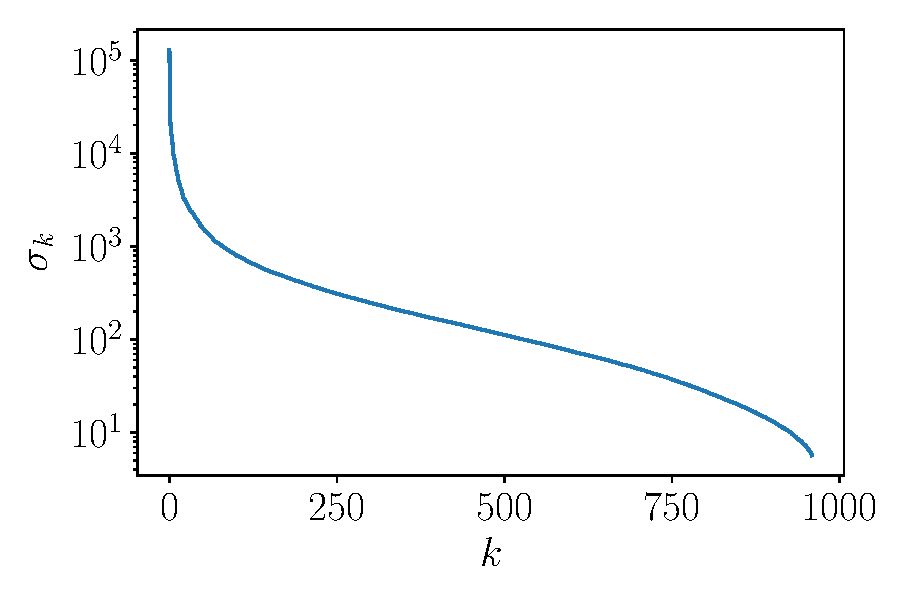
\includegraphics[width=0.99\linewidth]{ebookML_src/src/svd/singular_value.pdf}
\caption{}
\label{fig:26_3b}
% \label{fig:subim2}
\end{subfigure}
\begin{subfigure}{0.325\textwidth}
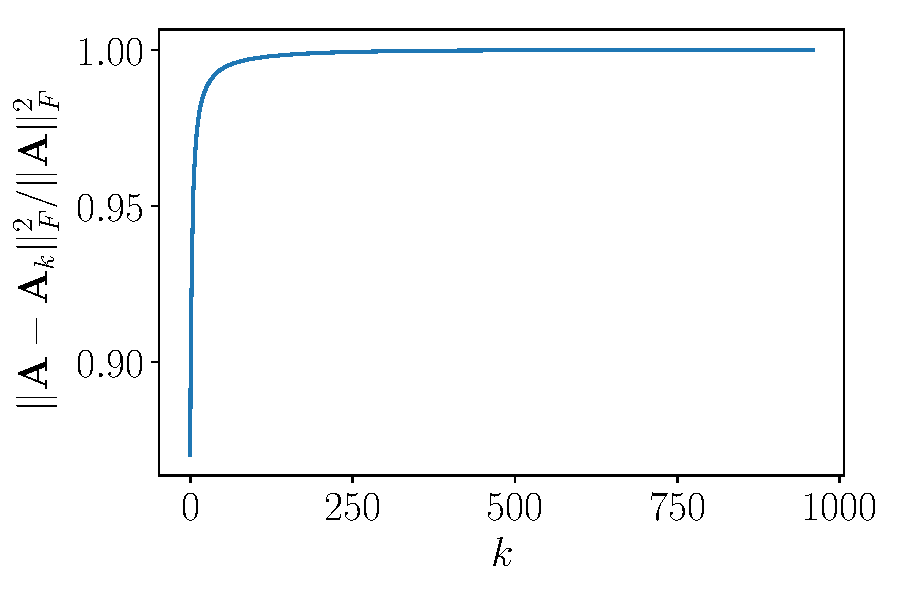
\includegraphics[width=0.99\linewidth]{ebookML_src/src/svd/energy_preserved.pdf}
\caption{}
\label{fig:26_3c}
% \label{fig:subim2}
\end{subfigure}
\\
\begin{subfigure}{0.325\textwidth}
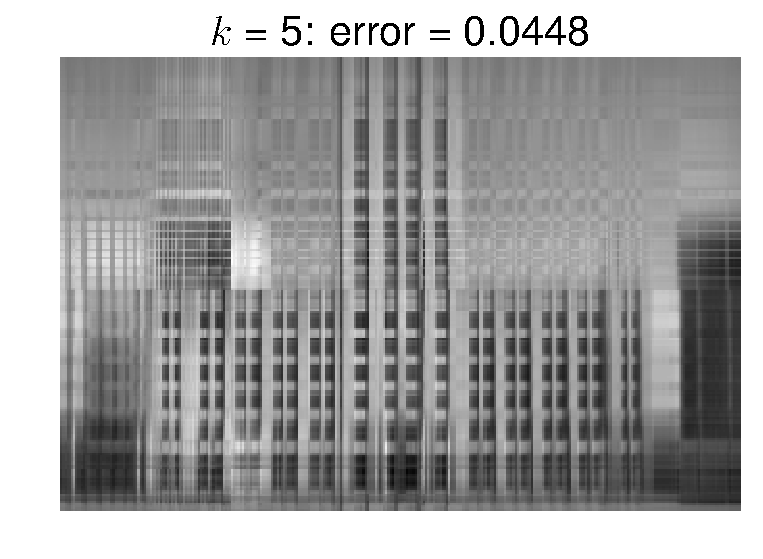
\includegraphics[width=0.99\linewidth]{ebookML_src/src/svd/image2_5.pdf}
\caption{}
% \label{fig:subim2}
\label{fig:26_3d}
\end{subfigure}
\begin{subfigure}{0.325\textwidth}
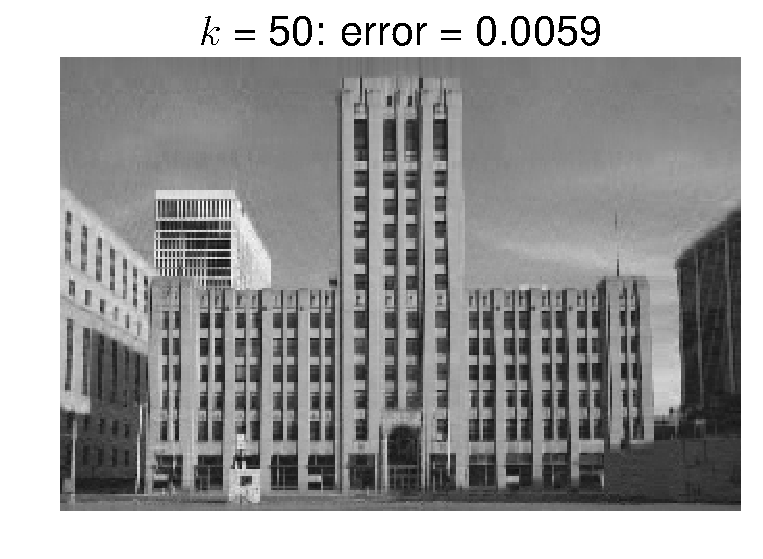
\includegraphics[width=0.99\linewidth]{ebookML_src/src/svd/image2_50.pdf}
\caption{}
% \label{fig:subim2}
\label{fig:26_3e}
\end{subfigure}
\begin{subfigure}{0.325\textwidth}
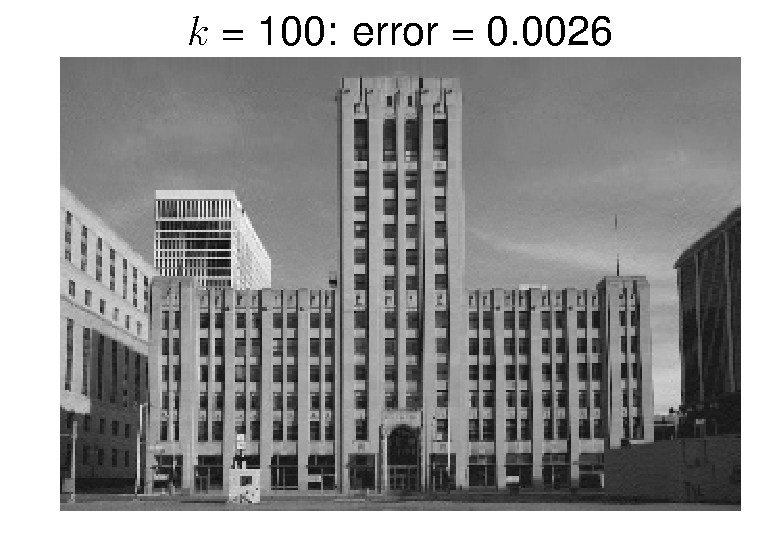
\includegraphics[width=0.99\linewidth]{ebookML_src/src/svd/image2_100.pdf}
\caption{}
\label{fig:26_3f}
% \label{fig:subim2}
\end{subfigure}
\caption{
Ví dụ về SVD cho ảnh. (a) Bức ảnh gốc là một ma trận cỡ $960
\times 1440$. (b) Các giá trị suy biến của ma trận ảnh theo thang đo logarit. Các giá trị suy biến giảm nhanh ở khoảng $k = 200$.
(c) Biểu diễn lượng thông tin được giữ lại khi chọn các $k$ khác nhau. Có
thể thấy từ khoảng $k = 200$, lượng thông tin giữ lại gần bằng 1.
Vậy ta có thể xấp xỉ ma trận ảnh này bằng một ma trận có hạng nhỏ hơn. (d),
(e), (f) Các ảnh xấp xỉ với $k$ lần lượt là 5, 50, 100.
}
\label{fig:26_3}
\end{figure}
% ******************************************************************************

Xét ví dụ trong Hình~\ref{fig:26_3}. Bức ảnh gốc trong Hình~\ref{fig:26_3a} là
một ảnh xám có
kích thước
$960\times 1440$ điểm ảnh. Bức ảnh này có thể được coi là một ma trận $\bA \in
\R^{960\times 1440}$. Có thể thấy rằng ma trận này có hạng thấp vì toà nhà có các tầng tương tự nhau, tức ma trận có nhiều hàng tương tự nhau.
Hình~\ref{fig:26_3b} thể hiện các giá trị suy biến sắp xếp theo thứ tự giảm dần
của ma trận điểm ảnh. Ở đây, các giá trị suy biến được biểu diễn trong thang logarit thập phân. Giá trị suy biến đầu tiên lớn hơn giá trị suy biến thứ 250 khoảng gần 1000 lần. Hình~\ref{fig:26_3c} mô tả chất lượng của việc xấp xỉ $\bA$ bởi
$\bA_k$ thông qua SVD cắt ngọn. Ta thấy giá trị này xấp xỉ bằng một tại $k =
200$. Hình~\ref{fig:26_3d}, \ref{fig:26_3e}, \ref{fig:26_3f} là các bức ảnh xấp
xỉ khi chọn các giá trị $k$ khác nhau. Khi $k$ gần 100, lượng thông tin mất đi hơn 0.3\%, ảnh thu được có chất lượng gần như ảnh gốc.


Để lưu ảnh với SVD cắt ngọn, ta lưu các ma trận $\mathbf{U}_k \in
\mathbb{R}^{m \times k}, \bSigma_k \in \mathbb{R}^{k \times k}, \mathbf{V}_k \in
\mathbb{R}^{n \times k}$. Tổng số phần tử phải lưu là $k(m + n + 1)$ với chú ý
rằng $\bSigma_k$ là một ma trận đường chéo. Nếu mỗi phần
tử được lưu bởi một số thực bốn byte thì số byte cần lưu là $4k(m + n + 1)$. Nếu so giá trị này với ảnh gốc có kích thước $mn$, mỗi giá trị là một số
nguyên một byte, tỉ lệ nén là
\begin{equation}
\frac{4k(m + n + 1)}{mn}
\end{equation}
Khi $k \ll m, n$, ta được một tỉ lệ nhỏ hơn 1. Trong ví dụ trên, $m =
960, n = 1440, k = 100$, tỉ lệ nén là xấp xỉ 0.69, tức đã tiết kiệm được
khoảng 30\% bộ nhớ.


% \subsection{Truncated SVD cho Recommendation System}
% Như đã nhắc ở Mục 1, SVD là một phương pháp Matrix Factorization, vì vậy, nó cũng hoàn toàn có thể được áp dụng vào bài toán Recommendation Systems như trong Chương \ref{cha:matrix_factorization}.

% Ý tưởng hoàn toàn tương tự, ta sẽ xấp xỉ Utility Matrix đã được chuẩn hoá (theo \textit{user-based} hoặc \textit{item-based}). Giá trị của ma trận xấp xỉ có rank nhỏ hơn chính là giá trị được dự đoán.

% Kết quả (RMSE) với cơ sở dữ liệu tương tự như Chương \ref{cha:matrix_factorization} là:
% \begin{itemize}
%     \item MovieLens 100k, user-based: 1.018 (tốt hơn so với 1.06 của Matrix Factorization).

%     \item MovieLens 100k, item-based: 1.014 (tốt hơn so với 1.05)

%     \item MovieLens 1M, item-based: 0.95 (tốt hơn so với 0.98)
% \end{itemize}

% Như vậy, Truncated SVD cho kết quả tốt hơn so với Matrix Factorization giải bằng Gradient Descent một chút.

% Một cách giải thích thú vị về mối liên quan giữa SVD và Utility Matrix với user-


\section{Thảo luận}

\begin{itemize}

\item Ngoài những ứng dụng nêu trên, SVD còn được áp dụng trong việc giải phương
trình tuyến tính thông qua giả nghịch đảo Moore Penrose
(\url{https://goo.gl/4wrXue}), hệ thống gợi ý~\cite{sarwar2000application}, giảm chiều dữ liệu~\cite{cybenko1989approximation}, \textit{khử mờ ảnh} (image deblurring)~\cite{hansen2006deblurring},
phân cụm~\cite{drineas2004clustering},...

\item Khi ma trận $\mathbf{A}$ lớn, việc tính toán SVD tốn nhiều thời
gian. Cách tính SVD cắt ngọn với $k$ như được trình bày trở nên không khả thi. Có một phương pháp lặp giúp tính
các trị riêng và vector riêng của một ma trận lớn một cách hiệu quả. Trong phương pháp này, ta
chỉ cần tìm $k$ trị riêng lớn nhất của $\mathbf{AA}^T$ và các vector riêng
tương ứng. Việc này giúp khối lượng tính toán giảm đi đáng kể. Bạn đọc có thể
tìm đọc thêm \textit{Power method for approximating eigenvalues}
(\url{https://goo.gl/PfDqsn}).


\item Mã nguồn trong chương này có thể được tìm thấy tại \url{https://goo.gl/Z3wbsU}.
\end{itemize}




\subsubsection{Đọc thêm}
\begin{enumerate}
\item \textit{Singular Value Decomposition - Stanford University} (\url{https://goo.gl/Gp726X}).

\item \textit{Singular Value Decomposition - Princeton} (\url{https://goo.gl/HKpcsB}).

\item \textit{CS168: The Modern Algorithmic Toolbox Lecture \#9: The Singular
Value Decomposition (SVD) and Low-Rank Matrix Approximations - Stanford}
(\url{https://goo.gl/RV57KU}).

\item \textit{The Moore-Penrose Pseudoinverse (Math 33A - UCLA)} (\url{https://goo.gl/VxMYx1}).
\end{enumerate}
